\begin{frame}{}
\begin{large}
\begin{center}
B.3 Long Run Risk Model
\end{center}
\end{large}
\end{frame}


\begin{frame}{Bansal and Yaron (2004)}\label{slide:BY2004}
\begin{footnotesize}
\begin{itemize}
	\item In this section, we present the model and approach proposed by \href{http://onlinelibrary.wiley.com/doi/10.1111/j.1540-6261.2004.00670.x/abstract}{Bansal and Yaron (2004)}: \textit{"Risks for the Long Run: A Potential Resolution of Asset Pricing Puzzles"}.
	\item A \href{https://jrenne.shinyapps.io/LRRModels}{web interface} present outputs of the approach. It also allows to simulate the model dynamics and to assess the influence of the parameterization.
	\item Bansal and Yaron have proposed two models: an homoskedastic one and an heteroskedastic one.
	\item Three risk sources in the aggregate consumption dynamics:
	\begin{itemize}
		\item Short-run risk risks in consumption (high frequency),
		\item Long-run risk risks in consumption (low frequency),
		\item Fluctuations in consumption uncertainty (heteroskedastic model).
	\end{itemize}
	\item Another key ingredient: Epstein-Zin preferences [Slide \ref{slide:EpsteinZin_def}].
	
	\vspace{.3cm}
	\item Let's begin with the homoskedastic model.
\end{itemize}
\end{footnotesize}
\end{frame}



\begin{frame}{Negative Long-Run Shock versus Short-Run Risk Shock}
%\begin{normalsize}
\begin{center}
Adverse Long-Run Shock:
\end{center}
		\begin{figure}
			\includegraphics[width=.85\linewidth]{figures/cartoon_lowerlonger.pdf}
		\end{figure}
%\end{normalsize}
\end{frame}


\begin{frame}{Bansal and Yaron (2004), homoskedastic}
\begin{footnotesize}
\begin{itemize}
	\item BY postulate the following dynamics for the economy:
	\begin{eqnarray*}
	x_{t+1} &=& \rho_x x_t + \phi_e \sigma e_{t+1}\\
	\Delta c_{t+1} = g_{t+1} &=& \mu + x_t + \sigma \eta_{t+1}\\
	g_{d,t+1} &=& \mu_d + \phi x_t + \phi_d \sigma u_{t+1},
	\end{eqnarray*}
	where $e_{t+1},\eta_{t+1},u_{t+1} \sim i.i.d. \mathcal{N}(0,1)$.
	\item $\mu + x_t$: conditional expectation of consumption growth ($g_t$);
	
	$g_{d,t}$: dividend growth rate ($\log(D_{t+1}/D_t)$).
	\item Processes $g_t$ and $g_{d,t}$ are exogenous. The model is solved by finding associated processes $r_{a,t}$ and $r_{m,t}$ that make the model internally consistent:
	These returns have to satisfy both Eqs. (\ref{eq:approxRa}) and (\ref{eq:sdfRa}).
	\item $z_t$ and $z_{m,t}$ are the {\color{blue}log price-consumption} and {\color{blue}price-dividend ratios}, respectively, i.e.:
	$$
	z_t = \log\left(\frac{P_{a,t}}{C_t}\right) \quad and \quad z_{m,t} = \log\left(\frac{P_{m,t}}{C_t}\right).
	$$
	%(Eq. \ref{eq:sdfRi} with $r_{i,t}=r_{m,t}$ for $z_{m,t}$)
	\item The price of a claim on aggregate consumption is not observable (return: $R_{a,t}$), contrary to the price of the market portfolio (return: $R_{m,t}$).
\end{itemize}
\end{footnotesize}
\end{frame}

\begin{frame}{Bansal and Yaron (2004), homoskedastic}
\begin{footnotesize}
\begin{itemize}
	\item Approach: (a) Posit that $z_t = A_0 + A_1 x_t$; (b) substitute the last expression into Eq. (\ref{eq:approxRa}) and (c) inject $r_{a,t+1}$ in Eq. (\ref{eq:sdfRa}).
	\item This yields to:
	\begin{equation}\label{eq:solABY1}
	A_1 = \frac{1- \dfrac{1}{\psi}}{1 - \kappa_1 \rho_x} \quad and \quad A_{1,m} = \frac{\Phi- \dfrac{1}{\psi}}{1 - \kappa_{1,m} \rho_x}.
	\end{equation}
	\item If the IES $\psi > 1$, then $A_1 > 0$. The price-consumption ratio increases with long-term growth.
	\item In this context, we have (from Eq. \ref{eq:sdfEZ}):
	\begin{eqnarray}\label{eq:mBY1}
	m_{t,t+1} - \mathbb{E}_t(m_{t,t+1}) &=& \left[  - \frac{\theta}{\psi} + \theta - 1\right] \sigma \eta_{t+1} \nonumber\\
	&&- (1 - \theta)\left[ \kappa_1 \left( 1 - \frac{1}{\psi}\right) \frac{\phi_e}{1 - \kappa_1 \rho_x} \right]\sigma e_{t+1}\nonumber\\
	&=& \lambda_{\eta} \sigma \eta_{t+1} - \lambda_{e} \sigma e_{t+1}.
	\end{eqnarray}
	(Note that $\lambda_{\eta} = -\gamma$.)
	\item The higher $\rho_x$, the higher $\lambda_{e}$.
\end{itemize}
\end{footnotesize}
\end{frame}

\begin{frame}{Bansal and Yaron (2004), homoskedastic}
\begin{footnotesize}
\begin{itemize}
	\item Consider any asset whose return is $r_{i,t}$, that is: $P_{i,t+1} = \exp(r_{i,t+1})P_{i,t}$. We must have:
	$$
	P_{i,t} = \mathbb{E}_t(\exp(m_{t,t+1})P_{i,t+1})= \mathbb{E}_t(\exp(m_{t,t+1}+r_{i,t+1})).
	$$
	\item Because the dynamics of the state vector is conditionally Gaussian, $m_{t,t+1}+r_{i,t+1}$ is conditionally Gaussian. Hence:
	\begin{eqnarray*}
	 1&=&\mathbb{E}_t\left(e^{m_{t,t+1}+r_{i,t+1}}\right)\\
	 &=&  \exp\left(\mathbb{E}_t(m_{t,t+1}+r_{i,t+1}) + \frac{1}{2}\mathbb{V}ar_t(m_{t,t+1}+r_{i,t+1})\right)\\
	 &=&  \exp\left(-r_{f,t}+\mathbb{E}_t(r_{i,t+1}) + \mathbb{C}ov_t(m_{t,t+1},r_{i,t+1}) + \frac{1}{2}\mathbb{V}ar_t(r_{i,t+1})\right).
	\end{eqnarray*}
	\item Therefore (particular case of  Eq. \ref{eq:MRCov}):
	\begin{equation}\label{eq:rp_cond}
	\mathbb{E}_t(r_{i,t+1}) -r_{f,t} = - \mathbb{C}ov_t(m_{t,t+1},r_{i,t+1}) - \frac{1}{2}\mathbb{V}ar_t(r_{i,t+1}).
	\end{equation}
	\item The risk premium results from the conditional covariance between $m_{t,t+1}$ and $r_{i,t+1}$, i.e. by the covariance of their innovations $m_{t,t+1} - \mathbb{E}_t(m_{t,t+1})$ and $r_{i,t+1} - \mathbb{E}_t(r_{i,t+1})$.
\end{itemize}
\end{footnotesize}
\end{frame}

\begin{frame}
\begin{scriptsize}
\begin{remark}[About the solution procedure]\label{remark:fixedpoint}
\begin{itemize}
	\item Eq. (\ref{eq:solABY1}) shows that the $A_i$s depends on the $\kappa_i$s.
	\item Eq. (\ref{eq:approxRa}) shows that the $\kappa_i$s depend on $\bar{z}$.
	\item Hence, in particular, $A_0 = f(\bar{z})$.
	\item But, in turn, since $z_t = A_0 + A_1 x_t$, we have $\bar{z}=A_0 + A_1 \bar{x}=A_0$.
	\item For the model to be internally consistent, we should have $\bar{z}=f(\bar{z})$. 
	\item[$\Rightarrow$] Fixed-point problem ($\bar{z}$ cannot be chosen arbitrarily).
\end{itemize}
\end{remark}

\begin{exampleblock}{Prices of Risk}
\begin{itemize}
	\item Let us consider an asset whose log return is $\beta\sigma\eta_{t+1}$ at date $t+1$, i.e. $r_{i,t+1}=\beta\sigma\eta_{t+1}$.
	\item Then Eq. (\ref{eq:rp_cond}) gives:
	$$
	\mathbb{E}_t(r_{i,t+1}) -r_{f,t} + \frac{1}{2}\beta^2\sigma^2 = - \lambda_{\eta}\beta\sigma^2.
	$$
	\item Because $\lambda_{\eta}=-\gamma<0$, $ - \lambda_{\eta}\beta\sigma^2$ is positive if $\beta\ge0$.
	\item $\lambda_\eta$ (resp. $\lambda_{e}$) measures the price of the "$\eta$ risk" (resp. the "$e$ risk").
	\item $\beta$ measures the exposure of stock $i$ to the shock $\eta_{t}$.
\end{itemize}
\end{exampleblock}
\end{scriptsize}
\end{frame}




%\begin{frame}{Bansal and Yaron (2004), homoskedastic}
%\begin{scriptsize}
%\begin{itemize}
%	\item Why do we care about $m_{t,t+1} - \mathbb{E}_t(m_{t,t+1})$?
%	
%	That is because of Eq. (\ref{eq:MRCov}): The excess return depends on the \textit{conditional} correlation between the returns and the s.d.f..
%	
%	\item The innovation in $m_{t,t+1}$ is sufficient to state about potential risk premium.
%	\item If an asset is conditionally independent from $m_{t,t+1}$, then its price incorporate no risk premium.
%	\item by contrast, if the asset returns are correlated to $m_{t,t+1} - \mathbb{E}_t(m_{t,t+1})$, then its price may incorporate risk premiums.
%	\item Neglecting (temporarily) for Jensen convexity effect and assume that $r_{f,t}$ is small, let us consider an asset whose return is $\sigma\eta_{t+1}$ at date $t+1$.
%	
%	In that case, the risk premium is approximately
%	$$
%	-\mathbb{C}ov_t\left(m_{t,t+1},\eta_t\right)=\lambda_\eta \sigma^2.
%	$$
%\end{itemize}
%\end{scriptsize}
%\end{frame}

\begin{frame}{Bansal and Yaron (2004), homoskedastic}
\begin{footnotesize}
\begin{itemize}
%	\item In this model, $r_{i,t}$ is Gaussian. Hence the risk premium on any asset $i$ is, approximately:
%	$$
%	\mathbb{E}_t(r_{i,t+1}-r_{f,t}) = -\mathbb{C}ov_t(m_{t,t+1}, r_{i,t+1}) - 0.5 \sigma_{r_i,t}^2.
%	$$
	\item Exploiting Eqs. (\ref{eq:approxRa}) (for $r_{m,t}$), (\ref{eq:solABY1}) and the model dynamics, we get:
	\begin{equation}\label{eq:rmErm}
	r_{m,t+1} - \mathbb{E}_t(r_{m,t+1}) = \phi_d  \underbrace{\sigma u_{t+1}}_{\mbox{not "priced"}} + \beta_{m,e}  \underbrace{ \sigma e_{t+1}}_{\mbox{"priced"}}
	\end{equation}
	where $\beta_{m,e} = \kappa_{1,m}\left(\phi - \dfrac{1}{\psi}\right)\dfrac{\phi_e}{1 - \kappa_{1,m} \rho_x}$.
	\item Then, using Eq. (\ref{eq:mBY1}), Eq. (\ref{eq:rp_cond}) gives, for $r_{i,t+1}=r_{m,t+1}$:
	\begin{equation}\label{eq:xsBYhomo}
	\mathbb{E}_t(r_{m,t+1} - r_{f,t}) = \beta_{m,e}\lambda_{e} \sigma^2 - 0.5 \mathbb{V}ar_t(r_{m,t}),
	\end{equation}
	where, by Eq. (\ref{eq:rmErm}), we have $\quad\mathbb{V}ar_t(r_{m,t})=(\beta_{m,e}^2+\phi_d^2)\sigma^2$.
	\item $\beta_{m,e}$ measure the exposure of stocks to the long-run risk shock $e_t$.
	\item The risk premium increases with $\rho_x$. Similarly, BY show that the volatility of the market return increases with $\rho_x$. [\href{https://jrenne.shinyapps.io/LRRModels}{web interface}].
	\item {\bf Remark}: constant $\sigma$ $\Rightarrow$ constant risk premium.
\end{itemize}
\end{footnotesize}
\end{frame}


\begin{frame}{Bansal and Yaron (2004), heteroskedastic}
		\begin{figure}
			\includegraphics[width=.8\linewidth]{figures/cartoon_volatility.pdf}
		\end{figure}
\end{frame}

\begin{frame}{Bansal and Yaron (2004), heteroskedastic}
\begin{footnotesize}
\begin{itemize}
	\item BY then introduce conditional volatility in the model [\href{https://jrenne.shinyapps.io/LRRModels}{web interface}]:
	\begin{eqnarray}\label{eq:BY_heteroscked}
	x_{t+1} &=& \rho_x x_t + \phi_e \sigma_t e_{t+1} \nonumber\\
	g_{t+1} &=& \mu + x_t + \sigma_t \eta_{t+1} \nonumber\\
	g_{d,t+1} &=& \mu_d + \phi x_t + \phi_d \sigma_t u_{t+1} \nonumber\\
	\sigma_{t+1}^2 &=& \sigma^2 + \nu_1(\sigma^2_t -\sigma^2) + \sigma_w w_{t+1},
	\end{eqnarray}
	where $e_{t+1},\eta_{t+1},u_{t+1},w_{t+1} \sim i.i.d. \mathcal{N}(0,1)$.
	\item Here, the posited solution for $z_t$ is:
	$$
	z_t = A_0 + A_1 x_t + {\color{red}A_2 \sigma^2_t}.
	$$
	\item $A_1$ is unchanged. $A_2$ is given by (similar form for $A_{2,m}$):
	$$
	A_2 = \frac{0.5 \left[ \left(\theta - \dfrac{\theta}{\psi}\right)^2 + (\theta A_1 \kappa_1 \phi_e)^2 \right]}{\theta(1 - \kappa_1 \nu_1)}.
	$$
	\item Remark \ref{remark:fixedpoint} also applies in this context.
\end{itemize}
\end{footnotesize}
\end{frame}

\begin{frame}{Bansal and Yaron (2004), heteroskedastic}
\begin{footnotesize}
\begin{itemize}
	\item The innovation of the s.d.f. is:
	\begin{eqnarray}\label{eq:mBY2}
 m_{t,t+1} - \mathbb{E}_t(m_{t,t+1}) = \lambda_{\eta} \sigma_t \eta_{t+1} - \lambda_{e} \sigma_t e_{t+1} - \lambda_{w} \sigma_w w_{t+1},
	\end{eqnarray}
	where $ \lambda_{w} = (1-\theta)A_2 \kappa_1$ and $\lambda_e$ and $\lambda_\eta$ are as in Eq. (\ref{eq:sdfEZ}).
	\item In the case of power utility ($\theta = 1$), the third term vanishes.
	\item The innovation of the market return is:
	\begin{equation}\label{eq:rmErmHetero}
	r_{m,t+1} - \mathbb{E}_t(r_{m,t+1}) = \phi_d  \underbrace{\sigma_t u_{t+1}}_{\mbox{not "priced"}} + \beta_{m,e}  \underbrace{ \sigma_t e_{t+1}}_{\mbox{"priced"}} + \beta_{m,w}  \underbrace{ \sigma_w w_{t+1}}_{\mbox{"priced"}}.
	\end{equation}
		\item Then Eq. (\ref{eq:rp_cond}) gives, for $r_{i,t+1}=r_{m,t+1}$:
	\begin{equation}\label{eq:xsBYhetero}
	\mathbb{E}_t(r_{m,t+1} - r_{f,t}) = \beta_{m,e}\lambda_{e} \sigma_t^2 + \beta_{m,w}\lambda_{w} \sigma_t^2 - 0.5 \mathbb{V}ar_t(r_{m,t}).
	\end{equation}
	\item Increase in volatility $\Rightarrow$ $\nnearrow$ excess returns. But this does not reflect increases in dividends $\Rightarrow$ equity prices $\ssearrow$ [Eq. \ref{eq:dp2}].
\end{itemize}
\end{footnotesize}
\end{frame}


\begin{frame}
	\begin{center}
	\begin{footnotesize}
	Increase in uncertainty $\Rightarrow$ Decrease in prices.
	\end{footnotesize}
	
	\vspace{.4cm}

	\includegraphics[width=.85\linewidth]{figures/cartoon_nooneknows.pdf}
	\end{center}
\end{frame}

\begin{frame}{Bansal and Yaron (2004), heteroskedastic}
\begin{footnotesize}
\begin{itemize}
	\item Compared the homoskedastic case [Eq. \ref{eq:xsBYhomo}], (a) the expected excess return is time-varying and (b) additional term = compensation for stochastic volatility risk in consumption.
	\item ratio of conditional risk premium to the conditional volatility of the market portfolio is time-varying (TV) $\Rightarrow$ TV Sharpe ratio.
	\item Maximal Sharpe ratio $\approx$ conditional volatility of the s.d.f. innovations. It is TV.
	
	\vspace{.5cm}
	\item The same kind of computation can be carried out for the return of the consumption claim ($r_{a,t}$). We get:
	\begin{equation}\label{eq:raEraHetero}
	r_{a,t+1} - \mathbb{E}_t(r_{a,t+1}) = \sigma_t \eta_{t+1} + \beta_{a,e}  \sigma_t e_{t+1} + \beta_{a,w}  \sigma_w w_{t+1},
	\end{equation}
	where $\beta_{a,e}=\kappa_1 A_1 \phi_e$ and $\beta_{a,w}=\kappa_1A_2$.
	\item Eq. (\ref{eq:rp_cond}) then gives:
	\begin{equation}\label{eq:xsaBYhetero}
	\mathbb{E}_t(r_{a,t+1} - r_{f,t}) = -\lambda_{\eta} \sigma_t^2 + \beta_{a,e}\lambda_{e} \sigma_t^2 + \beta_{a,w}\lambda_{w} \sigma_t^2 - 0.5 \mathbb{V}ar_t(r_{a,t}).
	\end{equation}
\end{itemize}
\end{footnotesize}
\end{frame}

\begin{frame}{Bansal and Yaron (2004), heteroskedastic}\label{slide:rfBY}
\begin{footnotesize}
\begin{itemize}
	\item The short term rate $r_{f,t}$ is such that $\exp(-r_{f,t})=\mathbb{E}_t(\exp(m_{t,t+1}))$.
	\item Using Eq. (\ref{eq:sdfEZ}), we have:
	$$
	\exp(-r_{f,t})=\mathbb{E}_t\left(\exp\left[\theta \log \delta - \frac{\theta}{\psi} g_{t+1} - (1-\theta) r_{a,t+1}\right]\right).
	$$
	\item We have:
	\begin{equation}
	r_{f,t} = - \theta \log (\delta) + \mathbb{E}_t\left(\frac{\theta}{\psi} g_{t+1}+ (1-\theta)r_{a,t+1} \right) - \frac{1}{2}\mathbb{V}ar_t\left(\frac{\theta}{\psi} g_{t+1} + (1-\theta) r_{a,t+1}\right),
	\end{equation}
	which, after computation, gives:
	\begin{equation}\label{eq:rfBY}
	r_{f,t} = - \log (\delta) + \frac{1}{\psi}\mathbb{E}_t(g_{t+1})+ \frac{1-\theta}{\theta} \mathbb{E}_t(r_{a,t+1}-r_{f,t}) - \frac{1}{2\theta}\mathbb{V}ar_t\left(m_{t,t+1}\right),
	\end{equation}
	 where $\mathbb{V}ar_t\left(m_{t,t+1}\right)$ is easily obtained from Eq. (\ref{eq:mBY2}) and $\mathbb{E}_t(r_{a,t+1}-r_{f,t})$ is given by Eq. (\ref{eq:xsaBYhetero}). \hyperlink{slide:rfBYappendix}{\beamergotobutton{formula}} 
	 \item Regressing $r_{f,t}$ on $g_{t+1}$ may give an estimate of $1/\psi$. BY: Time-varying intercept implies a downward bias on $\hat\psi$.
\end{itemize}
\end{footnotesize}
\end{frame}

\begin{frame}{Bansal and Yaron (2004), Results}
\begin{footnotesize}
\begin{itemize}
	\item The model-implied time-series properties are consistent with the data [Slide \ref{slide:tabI}].% [Note: simulation model without stochastic volatility]
	
	\item With persistent expected growth, the model is able to generate sizeable risk premiums, market volatility and fluctuations in price-dividend ratios [Slide \ref{slide:tabII}].
	\item Larger risk aversion increases the equity premium  [Slide \ref{slide:tabII}].
	\item In order to match data features, the IES has to be $>1$.
	\begin{itemize}
		\item 	Lowering the IES reduces the elasticity of asset prices to dividends, namely $A_{1,m}$ [Eq. \ref{eq:solABY1}], which reduces risk premia [\href{https://jrenne.shinyapps.io/LRRModels}{web interface}].
		\item If the IES is too small, this elasticity becomes negative: rise in dividend growth rate $\Rightarrow$ decreases in prices.
	\end{itemize}
	\item Lower part of the table in Slide \ref{slide:tabII}: i.i.d. growth rates. Then no correlation between dividend growth and consumption, and $\mathbb{E}_t(r_{m,t+1}-r_{f,t})=-1/2 \mathbb{V}ar_t(r_{m,t+1}) < 0$.
\end{itemize}
\end{footnotesize}
\end{frame}

\begin{frame}{Bansal and Yaron (2004), Results}
\begin{footnotesize}
\begin{itemize}
	\item While the time series properties of the model with small persistent expected growth are difficult to distinguish from a pure i.i.d. model, its asset-pricing implications are drastically different.
	\item Evidence in favor of the heteroskedastic model: In particular, relationship between the absolute values of innovations in consumption and the log price-dividend ratio (Table III in BY).
	\item Moments implied by the heteroskedastic model are shown in Table IV of BY [Slide \ref{slide:tabIV}].
	\item[$\Rightarrow$] Good fit of the data first and second moments.
	\item Volatility of the s.d.f.: the persistency of the expected growth rate is key (divided by two when $\rho_x$ is set to 0).
	\item The model replicates the way price-dividend ratios predict excess returns [Slide \ref{slide:tabVI}].
\end{itemize}
\end{footnotesize}
\end{frame}


\begin{frame}\label{slide:tabI}
\begin{scriptsize}
		\begin{figure}
			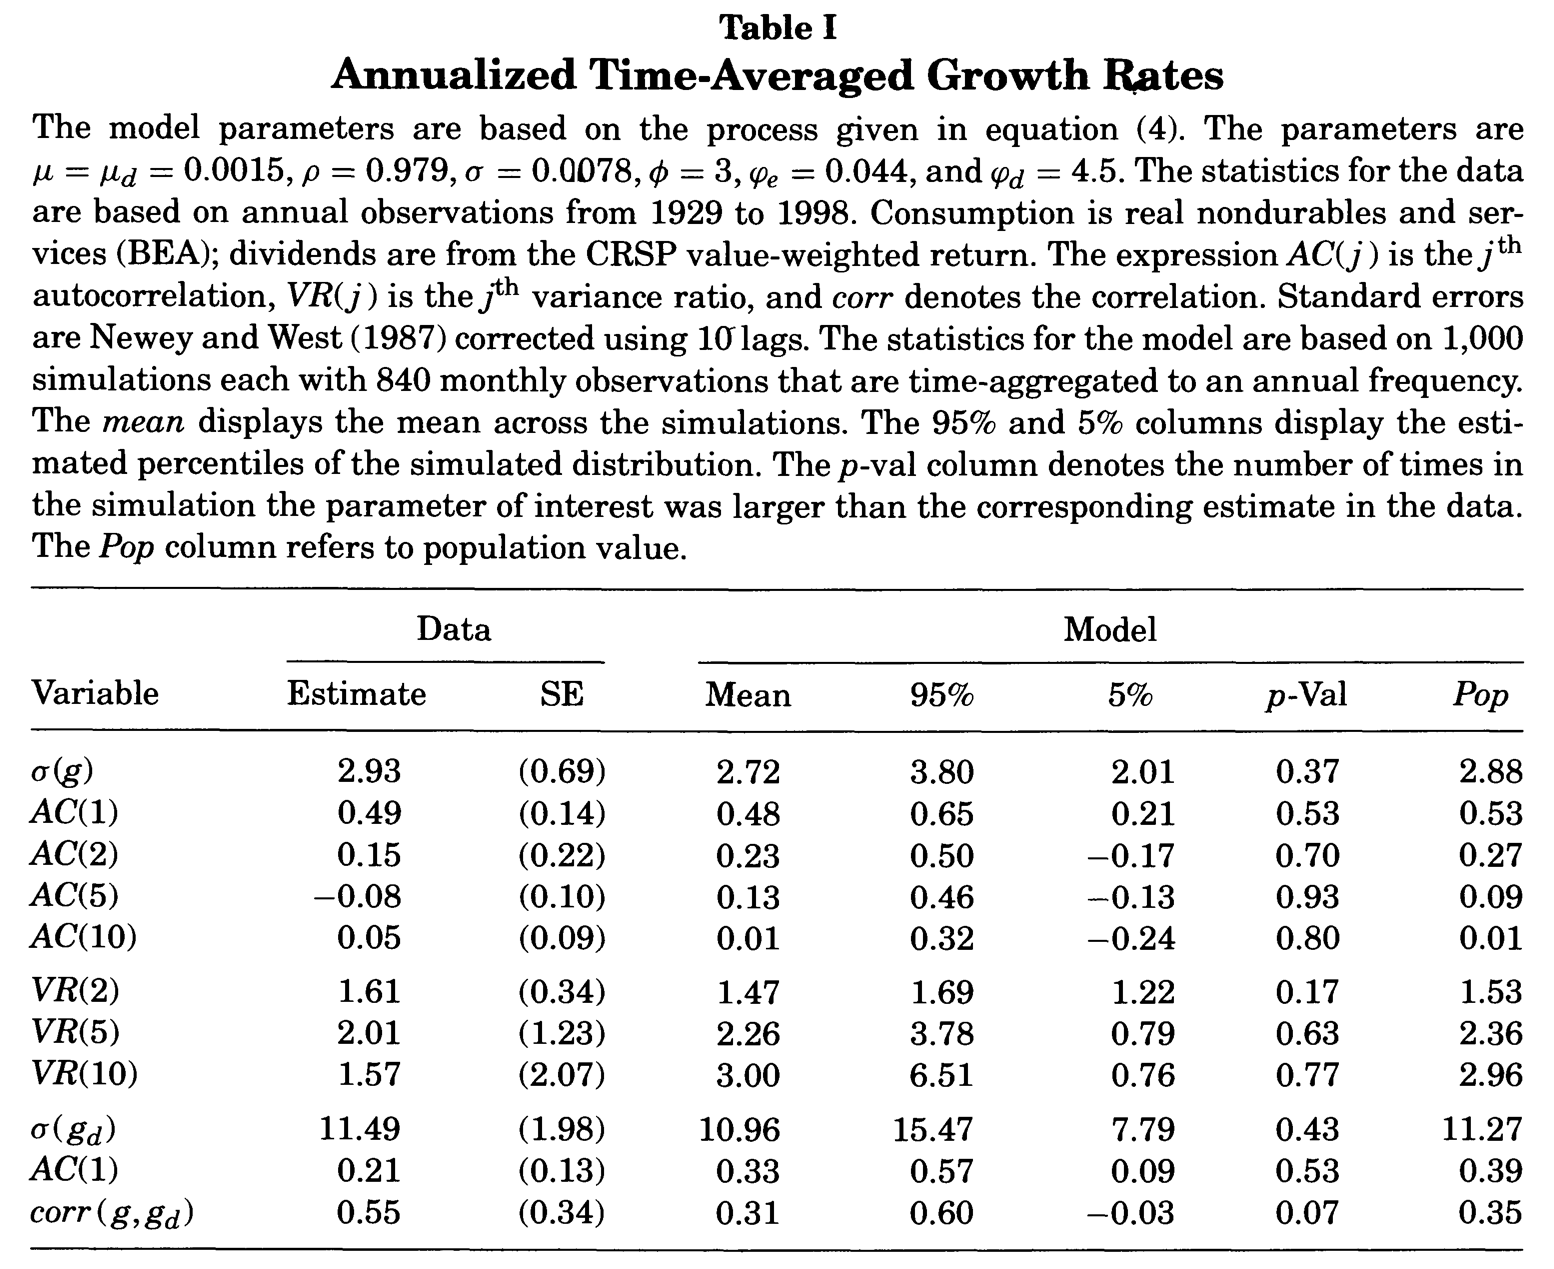
\includegraphics[width=.95\linewidth]{figures/table_BY1.pdf}
		\end{figure}
		\begin{tiny}
		\begin{center}
		Source: \href{http://onlinelibrary.wiley.com/doi/10.1111/j.1540-6261.2004.00670.x/abstract}{Bansal and Yaron (2004)}.
		\end{center}
		\end{tiny}
\end{scriptsize}
\end{frame}

\begin{frame}\label{slide:tabII}
\begin{scriptsize}
		\begin{figure}
			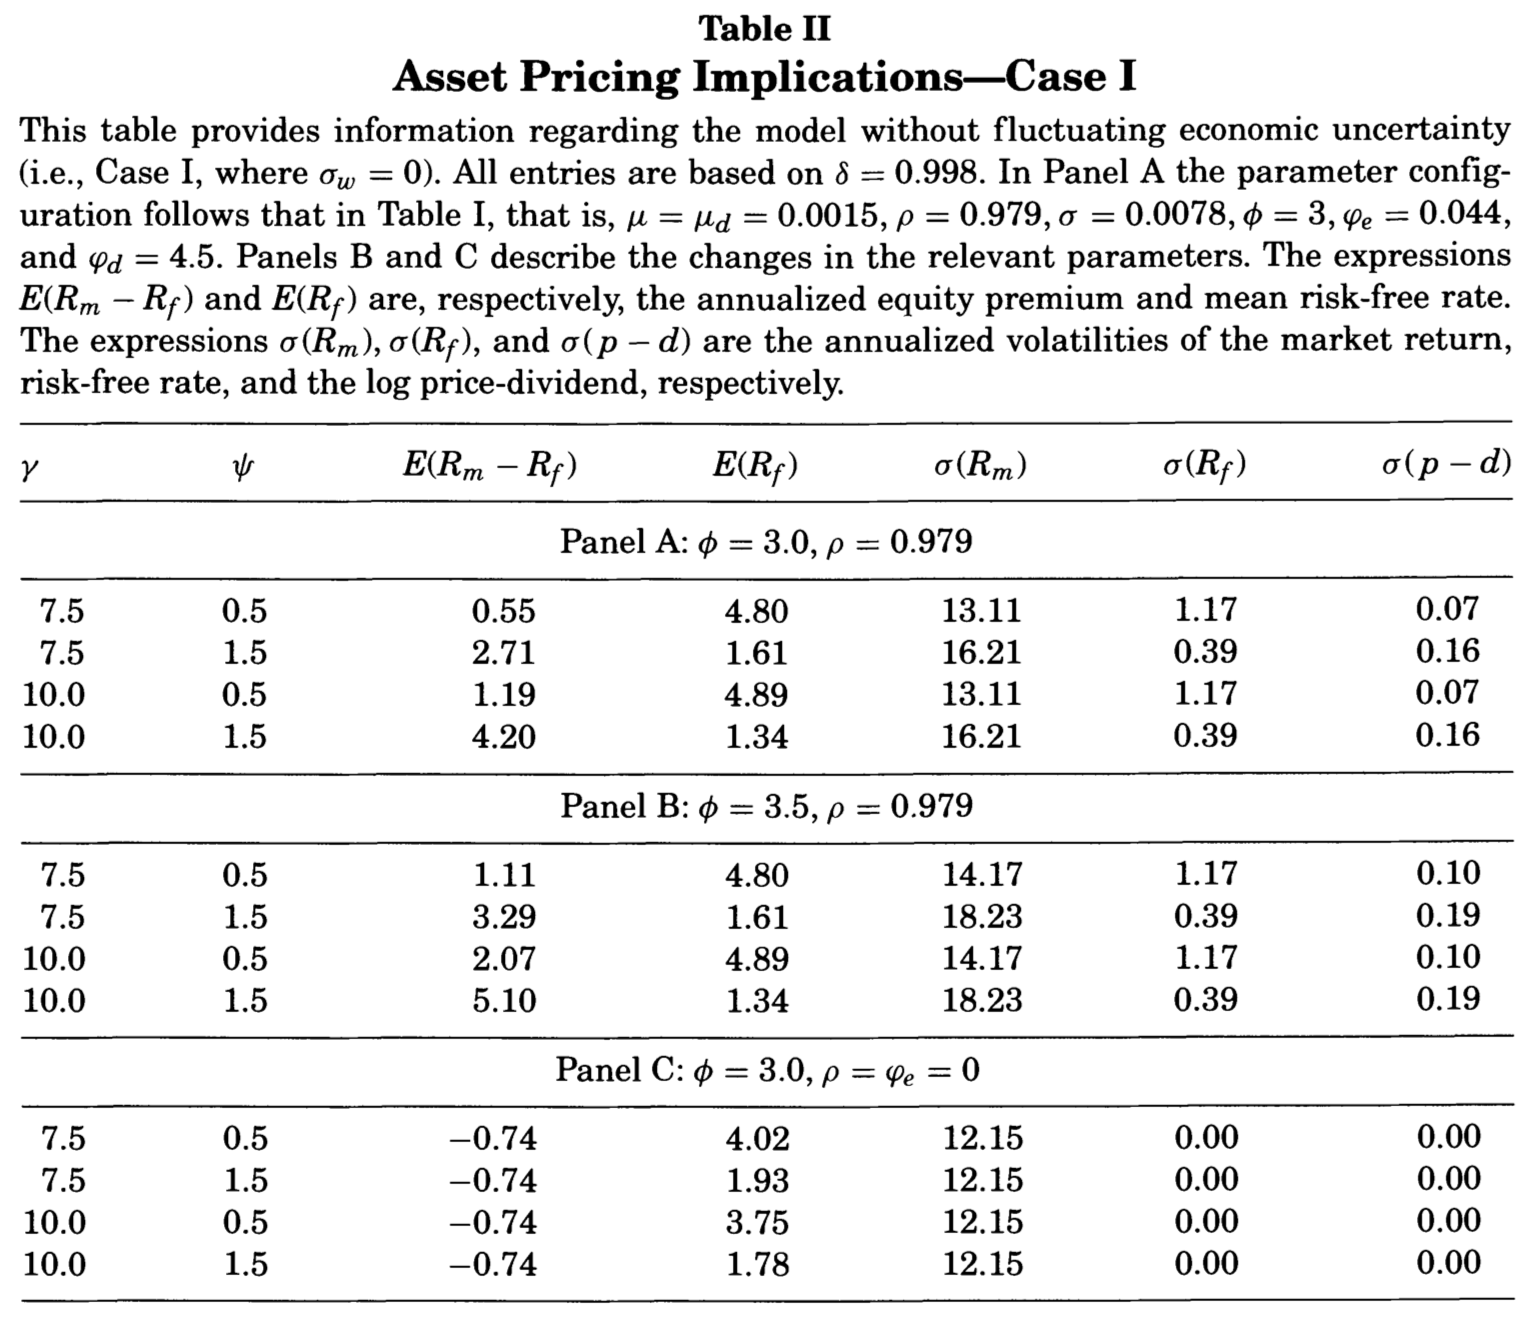
\includegraphics[width=.95\linewidth]{figures/table_BY2.pdf}
		\end{figure}
		\begin{tiny}
		\begin{center}
		Source: \href{http://onlinelibrary.wiley.com/doi/10.1111/j.1540-6261.2004.00670.x/abstract}{Bansal and Yaron (2004)}.
		\end{center}
		\end{tiny}
\end{scriptsize}
\end{frame}

\begin{frame}\label{slide:tabIV}
\begin{scriptsize}
		\begin{figure}
			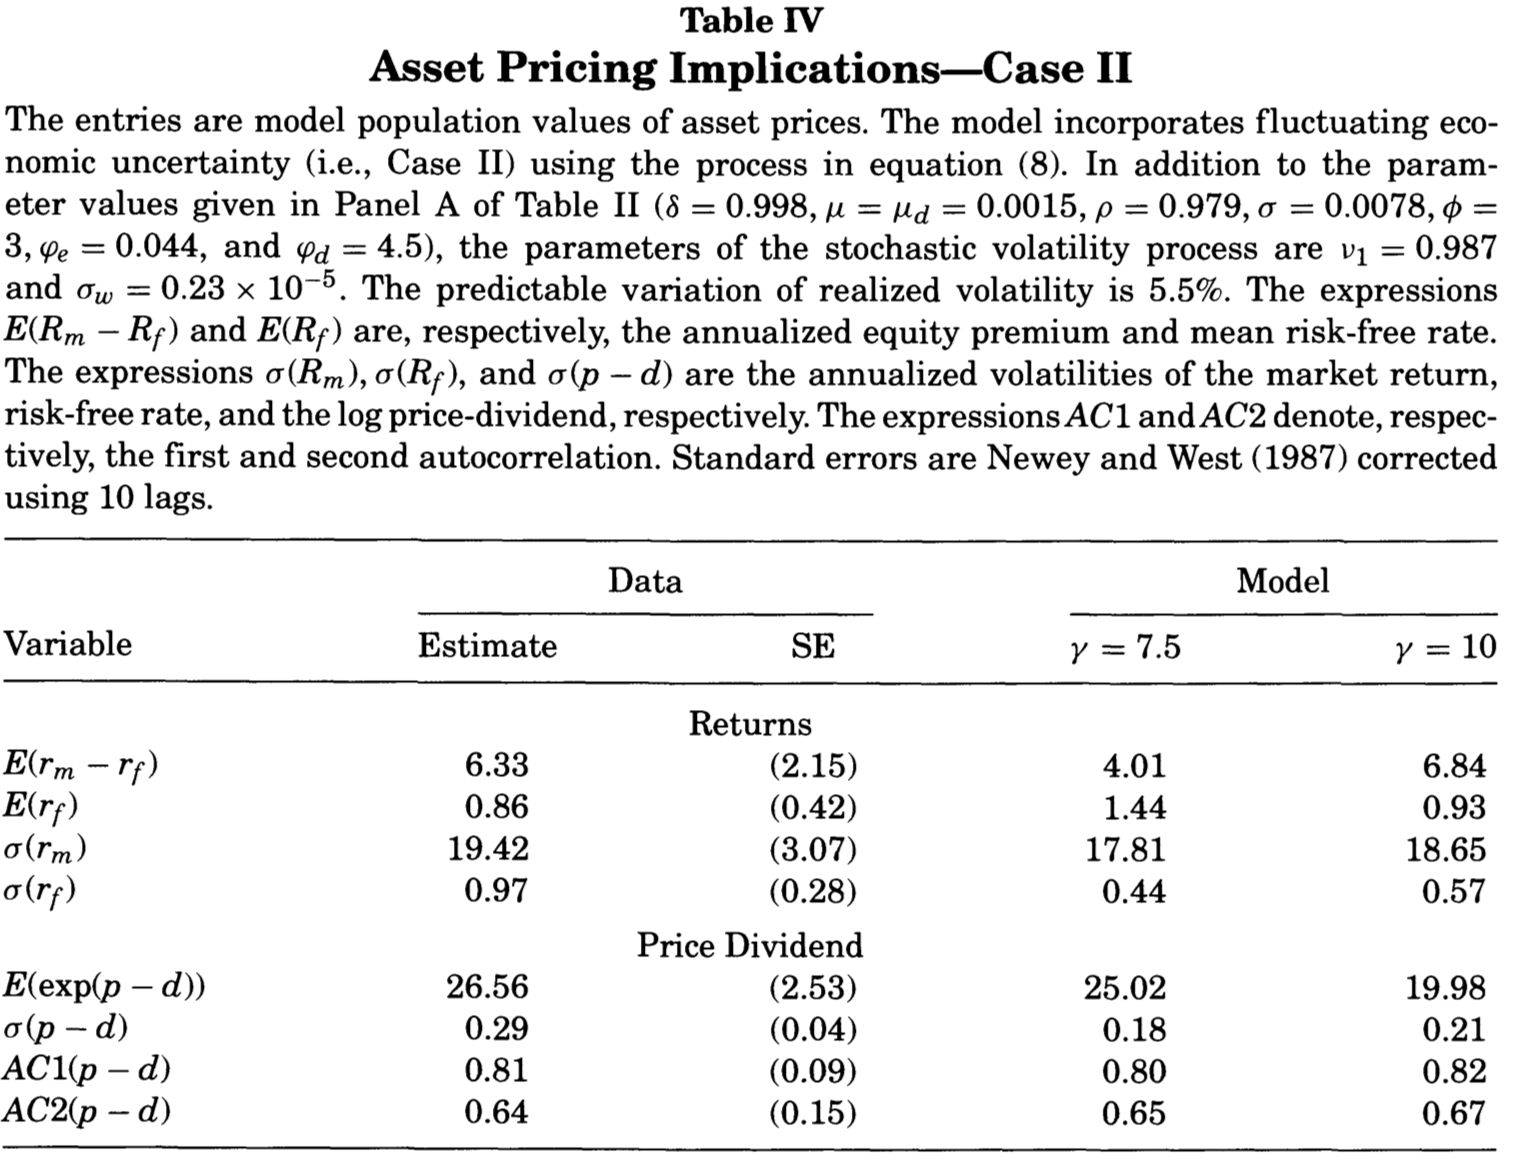
\includegraphics[width=.95\linewidth]{figures/table_BY4.pdf}
		\end{figure}
		\begin{tiny}
		\begin{center}
		Source: \href{http://onlinelibrary.wiley.com/doi/10.1111/j.1540-6261.2004.00670.x/abstract}{Bansal and Yaron (2004)}.
		\end{center}
		\end{tiny}
\end{scriptsize}
\end{frame}

\begin{frame}\label{slide:tabVI}
\begin{scriptsize}
		\begin{figure}
			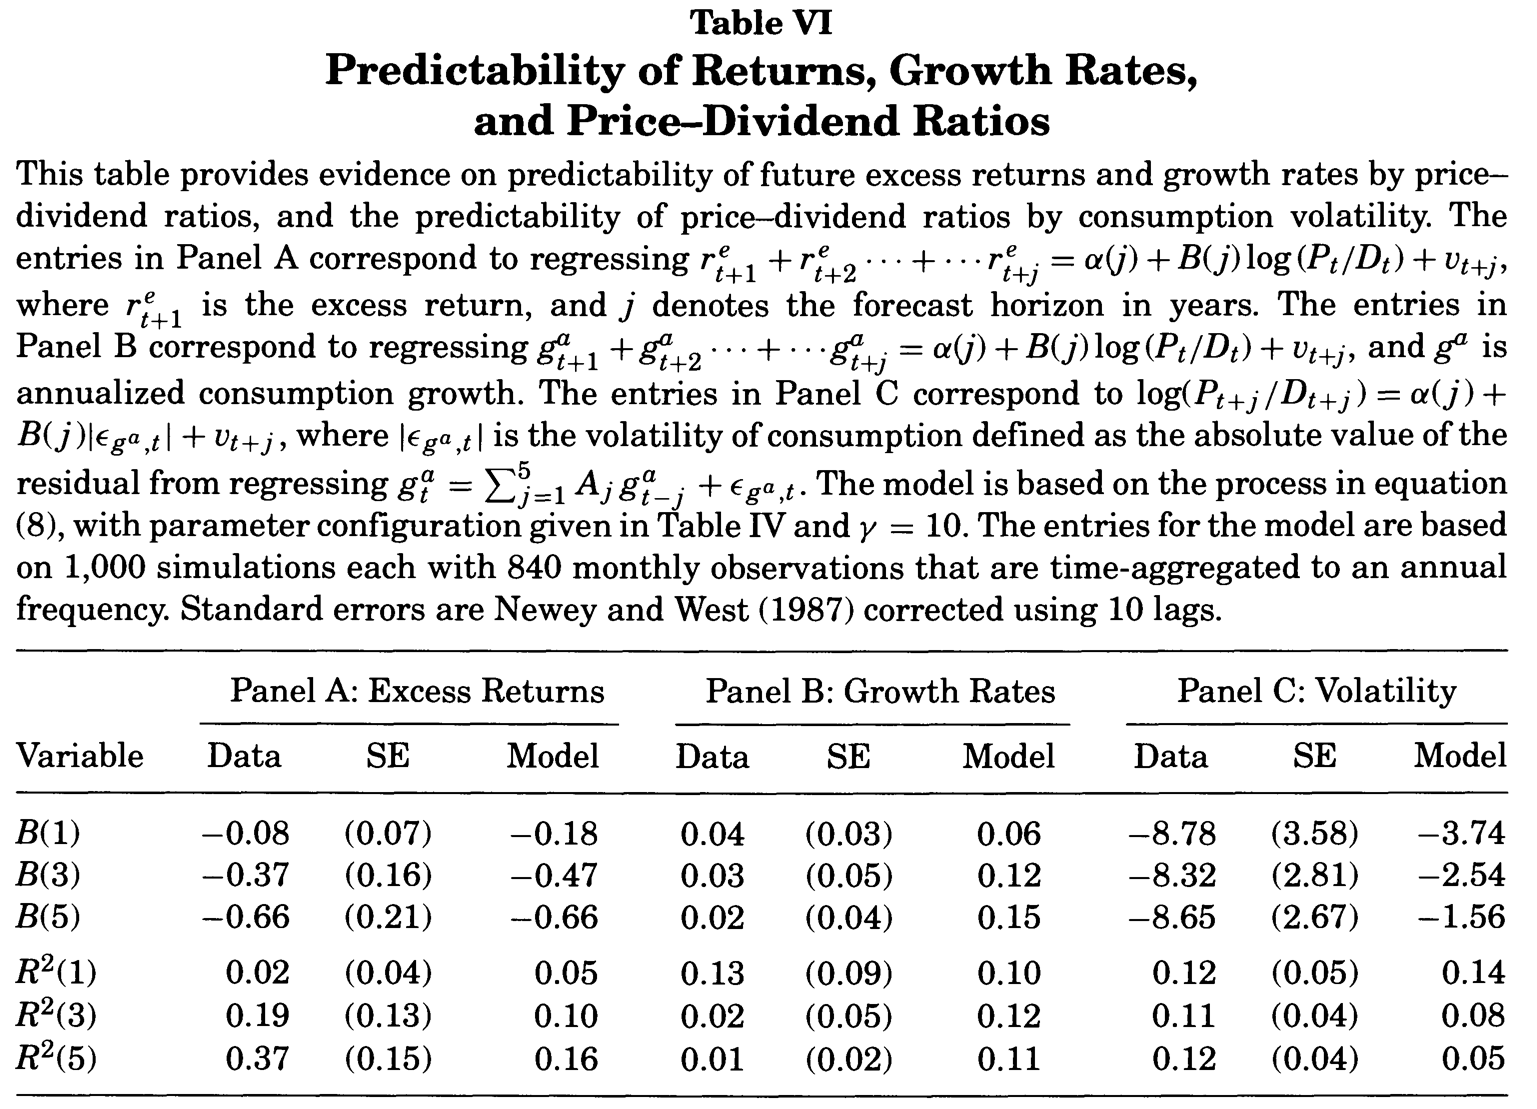
\includegraphics[width=.95\linewidth]{figures/table_BY6.pdf}
		\end{figure}
		\begin{tiny}
		\begin{center}
		Source: \href{http://onlinelibrary.wiley.com/doi/10.1111/j.1540-6261.2004.00670.x/abstract}{Bansal and Yaron (2004)}.
		\end{center}
		\end{tiny}
\end{scriptsize}
\end{frame}


\begin{frame}{Empirics of the LRR model: Bansal, Kiku and Yaron (2007)}
\begin{footnotesize}
\begin{itemize}
	\item \href{https://faculty.fuqua.duke.edu/~rb7/bio/BKY_09252007.pdf}{Bansal, Kiku and Yaron (2007)} show that their model is supported by cross-section data.
	\item Specifically, they want to see whether their model is able to reproduce the differences in excess returns for small/large and value/growth stocks [Slide \ref{slide:FamaFrench}].
	\item The model is slightly modified. The process followed by the dividend growth rate associated to stock $i$ is:
	$$
	g^{(i)}_{d,t+1} = \mu_d^{(i)} + \phi^{(i)} x_t + \pi^{(i)}\sigma_t \eta_{t+1} +  \phi^{(i)} \sigma u_{i,t+1}.
	$$
	\item Therefore, in this model, stock prices are also exposed to the short-run consumption growth rate $\eta_t$.
	
	\vspace{.3cm}
	\item Starting point: $r_{f,t}$ and $z_{m,t}$ are observable.
	\item Both variables are linear in $X_t=[x_t,\sigma_t^2]'$ [Slide \ref{slide:rfBY} for $r_{f,t}$].
	\item Hence, if one regress $\Delta c_{t+1}$ on $Y_t=[r_{f,t},z_t]$, the residuals are the same as those obtained when regressing $\Delta c_{t+1}$ on $X_t$, i.e. $\sigma_t \eta_{t+1}$.

\end{itemize}
\end{footnotesize}
\end{frame}


\begin{frame}{Extension: Bansal, Kiku and Yaron (2007)}
\begin{footnotesize}
\begin{itemize}
	\item Besides, $\mathbb{E}_t(\sigma_t^2 \eta_{t+1}^2)=\sigma_t^2$ is also a linear function of $X_t$. Therefore, the fitted values in the regression of $\sigma_t^2 \eta_{t+1}^2$ on $X_t$ provide estimates of $\sigma_t^2$.
	\item Once we have estimates of $x_t$ and $\sigma^2_t$, one can easily get estimates of their respective innovations, $e_t$ and $w_t$.
	\item For stock (or portfolio) $i$, BKY regress $r_{i,t+1}$ on $Y_t$. This provide them with estimates of the expected returns $\mathbb{E}_t(r_{i,t+1})$. The beta's of stock $i$ are then measured as the covariances between $r_{i,t+1}-\mathbb{E}_t(r_{i,t+1})$ and the estimates of the shocks $\eta_t$, $e_t$ and $w_t$ (divided by the variance of these shocks).
	\item 100 Fama-French porfolio (10 sizes and 10 book-to-market values); average excess returns are regressed on the beta's.
	\item[$\Rightarrow$] The three beta's explain about 84\% of the cross-sectional variation in mean returns.
	\item Macroeconomic interpretation of the Fama-French pricing factors (change of basis).
\end{itemize}
\end{footnotesize}
\end{frame}

\begin{frame}
\begin{scriptsize}
		\begin{figure}
			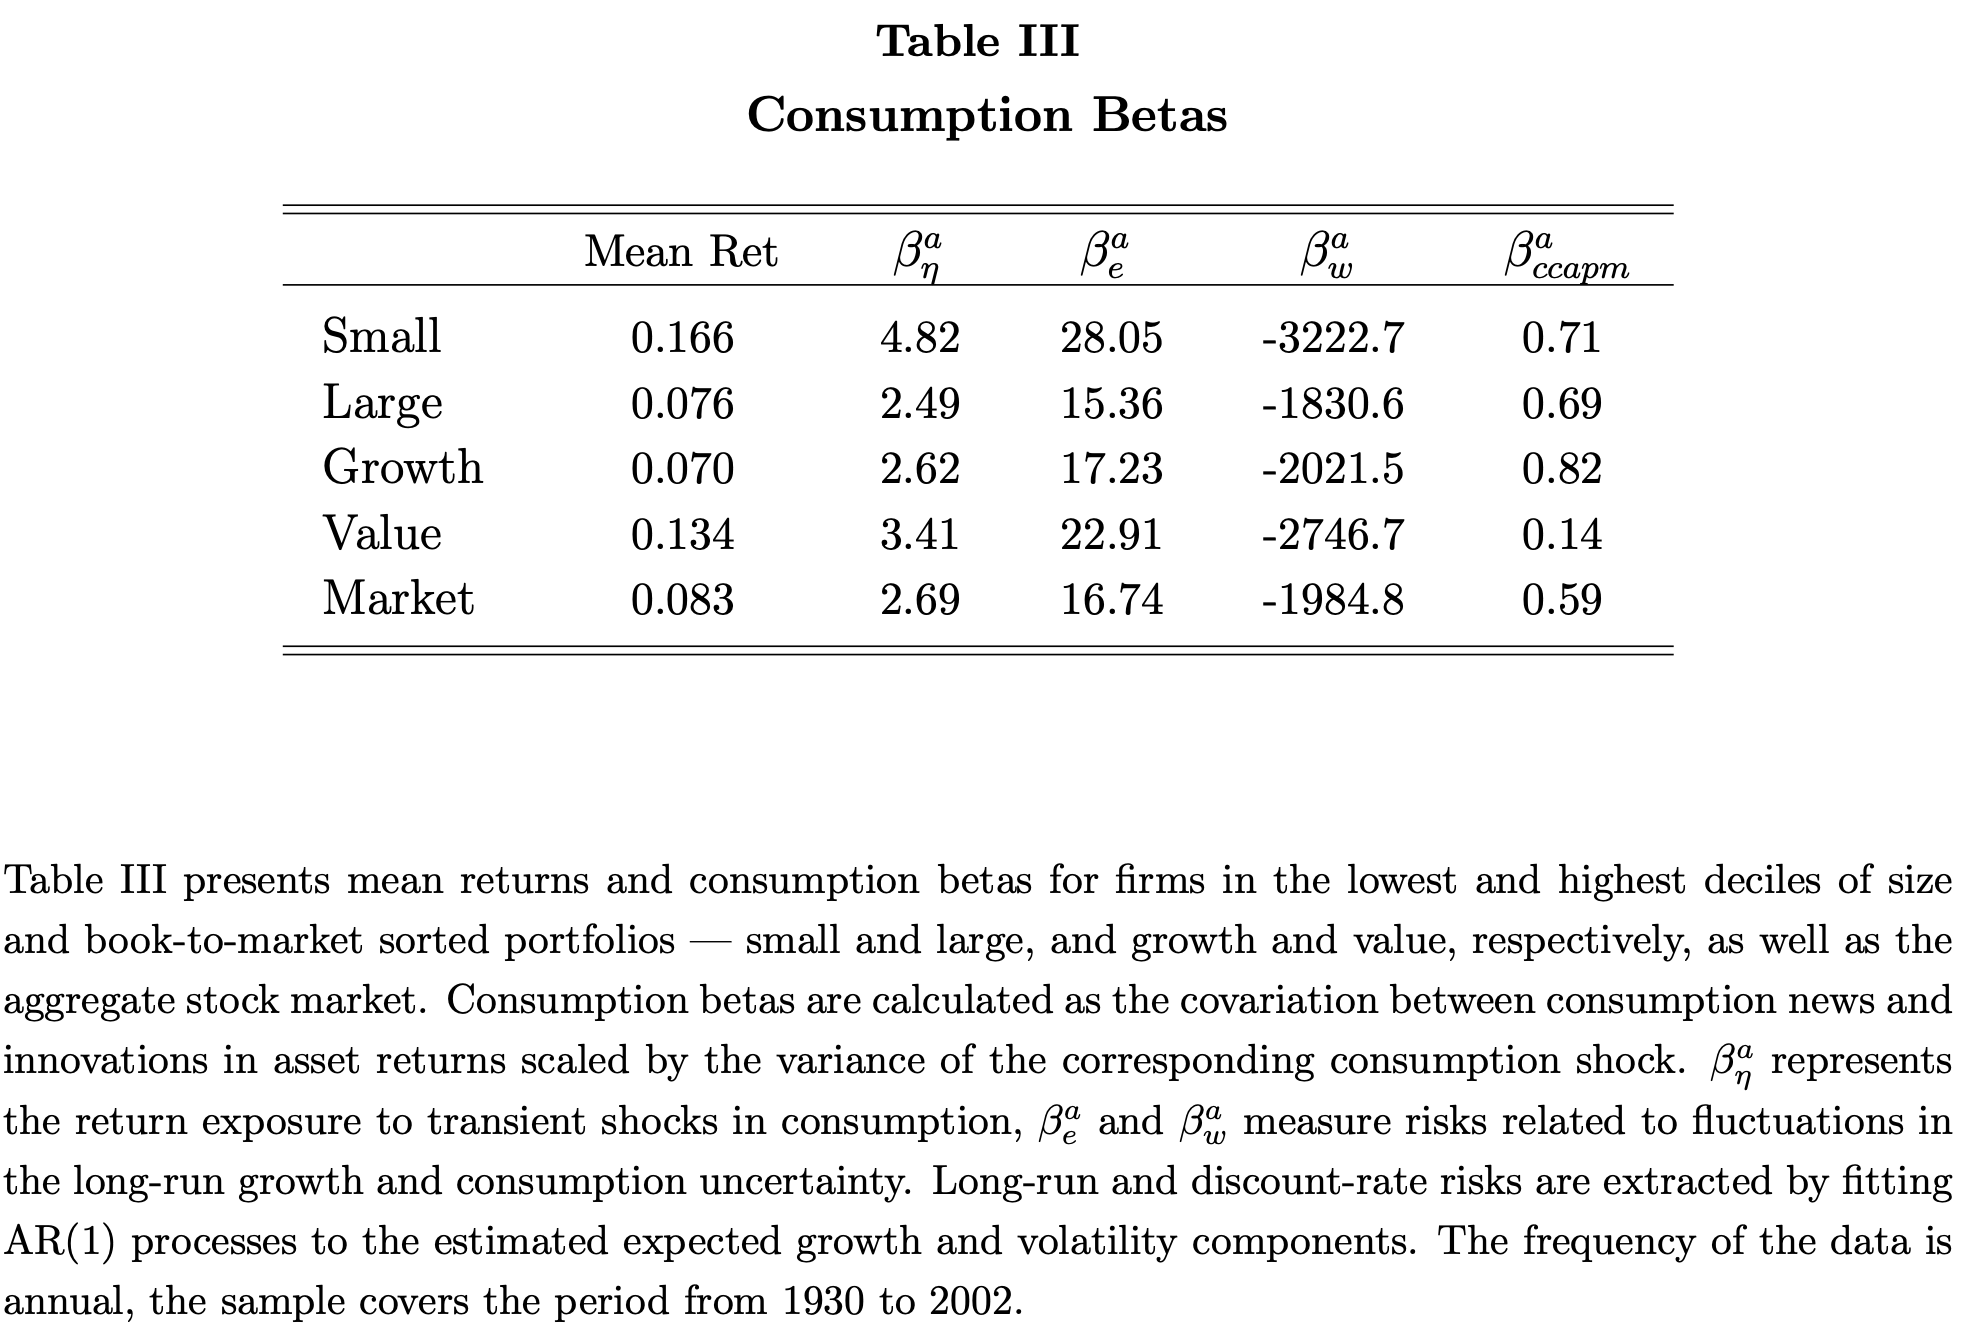
\includegraphics[width=.95\linewidth]{figures/table_BKY1.pdf}
		\end{figure}
		\begin{tiny}
		\begin{center}
		Source: \href{https://faculty.fuqua.duke.edu/~rb7/bio/BKY_09252007.pdf}{Bansal, Kiku and Yaron (2007)}.
		\end{center}
		\end{tiny}
\end{scriptsize}
\end{frame}

\begin{frame}
\begin{scriptsize}
		\begin{figure}
			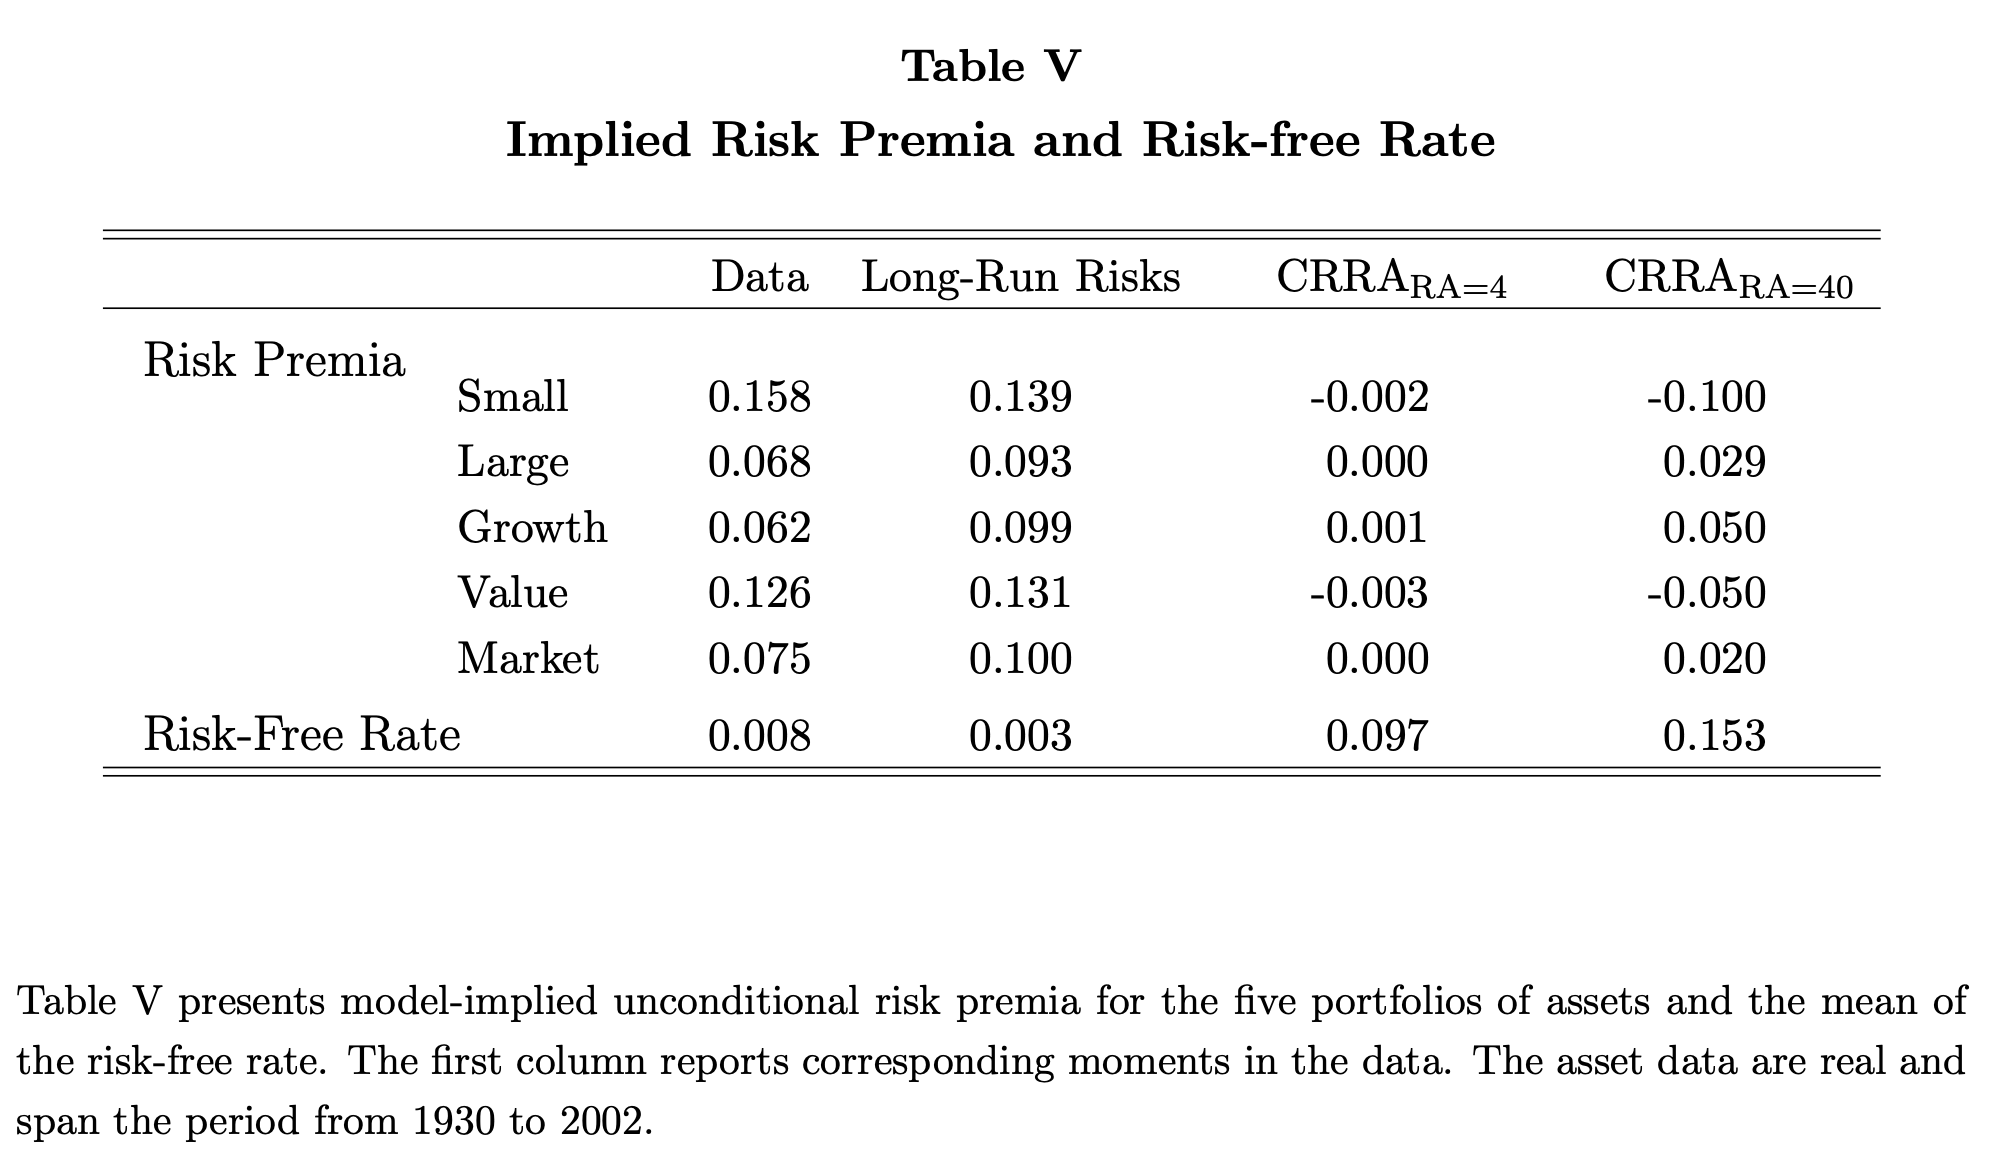
\includegraphics[width=.95\linewidth]{figures/table_BKY2.pdf}
		\end{figure}
		\begin{tiny}
		\begin{center}
		Source: \href{https://faculty.fuqua.duke.edu/~rb7/bio/BKY_09252007.pdf}{Bansal, Kiku and Yaron (2007)}.
		\end{center}
		\end{tiny}
\end{scriptsize}
\end{frame}





